To validate the hidden Markov model implmentation, 
we use both simulated examples
to build intuition, alongside
simulation-based calibration \citep{talts2018,modrak2023}.
Simulation-based calibration leverages the self-consistency
of the Bayesian joint distribution of parameters and
data: fitting a Bayesian model to datasets generated
from its prior predictive distribution and averaging 
over datasets should return the prior distribution.
Specific simulated examples, in addition, helps
build intuition about model dynamics.

\subsection{Simulation-based calibration}
Focusing on the base HMM model variant, 1000 
full-triangles with $N = M = 10$ were generated
from the prior predictive distribution, and the
HMM model fit to each upper diagonal $\mathcal{Y}$.
The prior distributions were the same as in
equation (\ref{eq:hmm}), except for the priors
on $(\gamma_{1}, \gamma_{2})$, which were 
given more informative normally-distributed priors
with locations and scales of $(-3, -0.25)$ and
$(-1, 0.1)$, respectively. Due to the
multiplicative autoregressive forms in the
location and scales of the likelihood in
equation (\ref{eq:hmm}), particularly
large values for $\sigma$ can cause overflow
in the sampled data.

Each model was summarised by
calculating the rank statistics of quantities
of interest.
The rank statistic is the number of times a
simulated value is greater than the posterior values,
and should be approximately uniformly distributed
if the model has been implemented correctly and is
unbiased \citep{talts2018}. To reduce the autocorrelation
in the posterior distributions, the posteriors were
thinned to every 10th posterior draw.
Rank statistics
were calculated for each parameter in the HMM model,
as well as the joint log likelihood and
an the ultimate loss prediction at data point
$(i=1, j=10)$, since \cite{modrak2023} recommend
using test quantities that average over the entire
data space in evaluating SBC.

No problems with model calibration were found using simulation-based
calibration (Figure \ref{fig:sbc}),
with all histograms matching the assumptions of
uniformity. However, 10 models were removed for poor
convergence, which typically occurred when the simulated
link ratios from the body process were
higher than values expected from real loss triangles. 
Given this occurred rarely, the priors were left
unchanged, although suitable prior distributions
for Bayesian chain ladder models is an area
with a dearth of literature.
For the 990 models, 
the average classification accuracy of the recovered latent
state values $\bm{z}$, across
both training and test data, was 97\% with a 
95\% highest density interval (i.e. the 95\% most
likely values) of [91, 100].

\begin{figure}
    \centering
    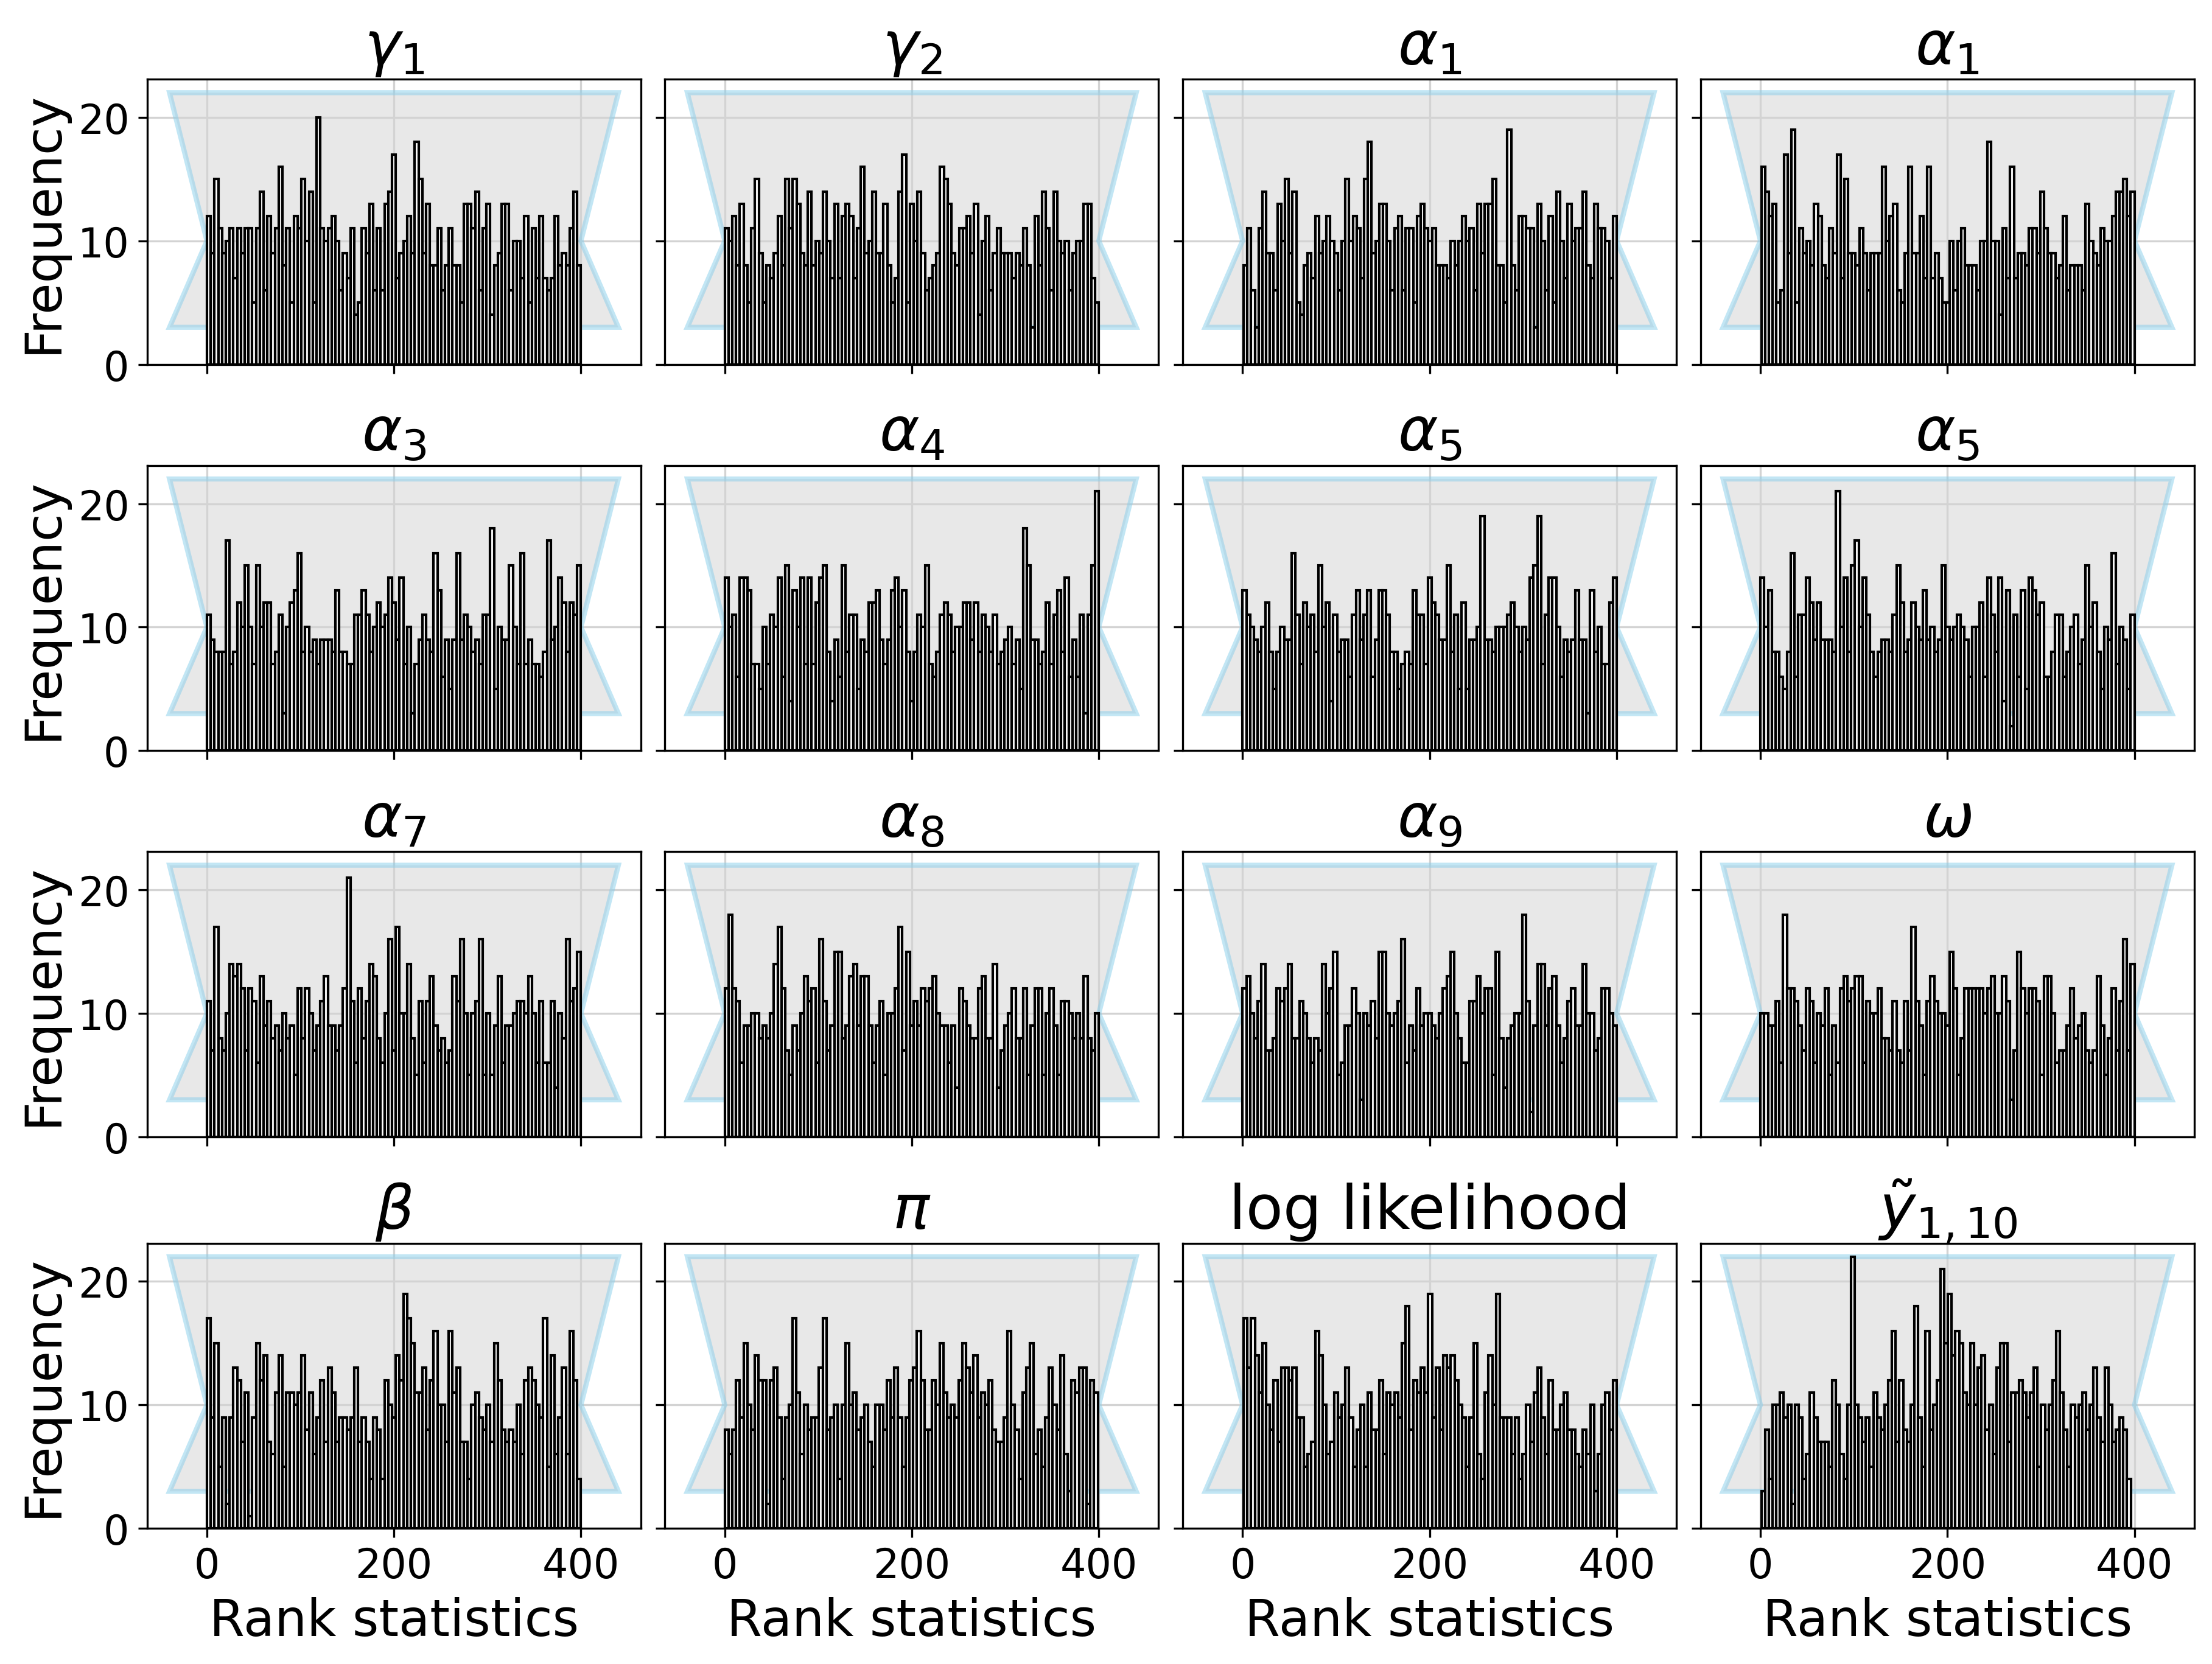
\includegraphics[scale=0.45]{\figures/ranks}
    \caption{
		Histograms of simulation-based calibration
		rank statistics for the HMM model, 
        with the 99\% percentile
        interval from a discrete uniform distribution
        shown in the grey shaded band.
        Each histogram shows a key model parameter,
        and the final two panels show the ranks
        for the joint log
        likelihood and the first ultimate loss
        distribution.
        For each model, we sampled
        4000 draws from the posterior distribution,
        and thinned the samples by 10 to remove any
        autocorrelation, meaning a maxmimum rank statistic
        of 400. Of the 1000 models,
        10 were removed due to poor convergence.
    }
	\label{fig:sbc}
\end{figure}

\subsection{Simulated example}
To build intuition for the two models,
Figure \ref{fig:numerical} shows a numerical
simulation of data from a HMM model,
and the results for the HMM model
(panel A), the latent change-point
model (panel B), and the
two-step model (panel C).
As shown by the ELPD values above each
plot with available test data (experience
periods two to ten), 
the HMM variant outperforms
the latent change-point and two-step approach
in all
experience periods except the second.
For the two-step process, the chosen value $\tau = 6$
matches the HMM data-generating process
closely for that experience period, 
resulting in higher accuracy. 
The latent change-point model detected the most
likely switch-over point at $\tau = 4$ with probability
46.5\%, but the relatively smooth dynamics of the
second experience period and 9 training data points
results in accurate estimation and predictions. 
In the remaining experience
periods, however, the two-step and latent change-point approaches
generalise poorly.
For instance, the third experience period (third row)
shows that the consequences of the $\tau$ values results
in over-estimation of losses in the latent change-point
and two-step approaches.
Similarly, the fifth experience period (fifth row)
shows a case where the tail model is never
entered by the HMM process, and the
latent change-point and two-step processes
consequently under-estimate true losses.
This example illustrates that
if $\tau$ is chosen correctly, there is sufficient
data available for model training,
and the data is typically well-behaved,
the two-step and latent change-point approaches 
can provide more exact predictions.
However, if experience periods differ in their
body-to-tail switch-over dynamics,
which is highly expected, then overall
performance suffers due to
growing generalisation error.

\begin{figure}
    %\hspace{-1.8cm}
    \vspace{-1.25cm}
    \centering
    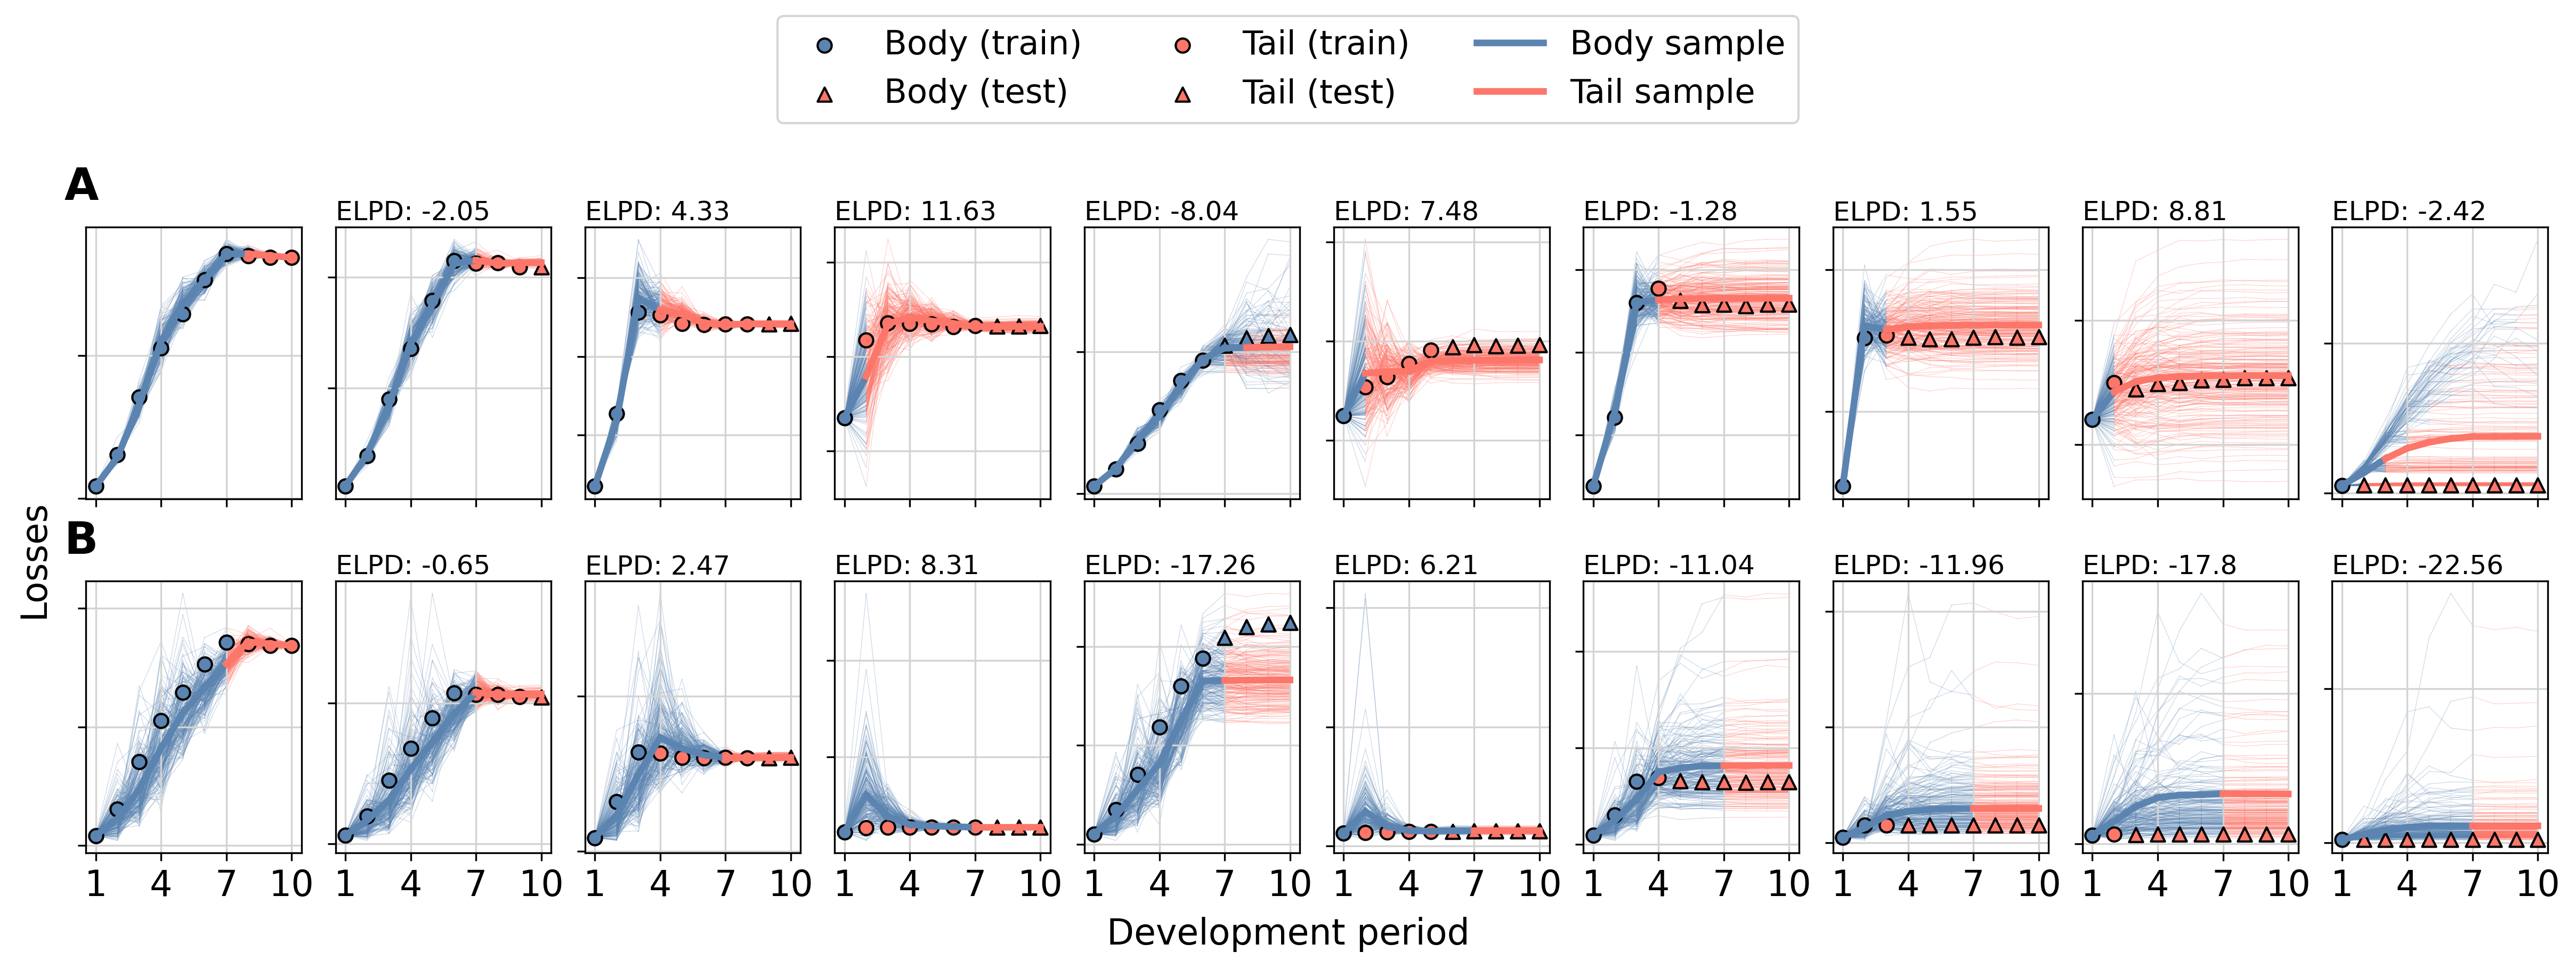
\includegraphics[scale=0.45]{\figures/numerical}
    \caption{
        Comparison of the HMM (panel A), 
        latent change-point (panel B)
        and two-step (panel C) models on ten accident
        periods (rows) of data simulated from
        the HMM model.
        The true losses
        are shown as points, with colours
        identifying true
        body (blue) or tail (orange) status.
        Circles denote training data and
        triangles test data. Thin 
        lines are samples from the posterior
        predictive distributions, coloured
        by latent state, and the thicker
        line shows the posterior mean.
        The ELPDs on the test data
        points in each experience period
        are shown above each plot.
        The two-step model was fit
        assuming $\tau = 6$ and
        $\bm{\rho} = (6, 10)$.
    }
	\label{fig:numerical}
\end{figure}
